\subsection{Základní stavy lehkých prvků}
Hamiltonián atomu s protonovým číslem $Z$ je
\begin{subequations}
    \begin{align}
        \operator{H}&=\operator{T}+\operator{V}^{(1)}+\operator{V}^{(2)},\\
        \operator{T}&=\sum_{j=1}^{Z}\operator{t}_{j}=\sum_{j=1}^{Z}\frac{\vectoroperator{p}_{j}^{2}}{2M},\\
        \operator{V}^{(1)}&=\sum_{j=1}^{Z}\operator{v}^{(1)}_{j}=-Z\gamma\sum_{j=1}^{Z}\frac{1}{\operator{r}_{j}},\\
        \operator{V}^{(2)}&=\sum_{j<k}\operator{v}^{(2)}_{jk}=\gamma\sum_{j<k}\frac{1}{\abs{\vectoroperator{r}_{j}-\vectoroperator{r}_{k}}},
    \end{align}        
\end{subequations}
kde $\operator{T}$ je kinetická energie elektronů v atomovém obalu, $\operator{V}^{(1)}$ popisuje interakci elektronů s atomovým jádrem a $\operator{V}^{(2)}$ vzájemnou elektrostatickou interakci mezi elektrony.
Uvažujte jen elektronové stupně volnosti, pohyb jádra zanedbejte.

Počítejte v bezrozměrných atomových jednotkách $\hbar=\gamma=M=1$.
Jednotka energie pak je $2E_{0}$, kde $E_{0}=13,\!6\,\mathrm{eV}$ je ionizační energie atomu vodíku.

Za jednočásticovou bázi $\ket{a}$ zvolte bázi vodíkupodobného atomu s nábojem jádra $Z$, kde $a=\{n,l,m,s\}$ (hlavní, orbitální a magnetické kvantové číslo a projekce spinu elektronu $s=\pm\frac{1}{2}$)
V ní je jednočásticová část Hartree-Fokovy rovnice diagonální,
\begin{align}
    \matrixelement{a}{\operator{t}_{j}+\operator{v}^{(1)}_{j}}{c}&=-\frac{Z^{2}}{2n^{2}}\delta_{ac}.
\end{align}
Pro dvoučásticovou část je potřeba vyjádřit maticové elementy
\begin{equation}
    \matrixelement{ab}{\vectoroperator{v}^{(2)}}{cd}
        =\matrixelement{ab}{\frac{1}{\abs{\vectoroperator{r}_{1}-\vectoroperator{r}_{2}}}}{cd}
        =\int\d^{3}\,r_{1}\,\d^{3}r_{2}\psi_{a}^{*}(\vector{r}_{1})\psi_{b}^{*}(\vector{r}_{2})\frac{1}{\abs{\vector{r}_{1}-\vector{r}_{2}}}\psi_{c}(\vector{r}_{1})\psi_{d}(\vector{r}_{2}),
    \label{eq:HFMatrixElement}
\end{equation}
kde
\begin{equation}
    \psi_{a}(\vector{r})\equiv\psi_{nlm}(\vector{r})\chi_{s}
        =R_{nl}(r)Y_{m}^{(l)}(\theta,\phi)\chi_{s}
\end{equation}
Provedeme následující zanedbání:
\begin{itemize}
    \item Omezíme se na $s$-orbitaly, tj. na orbitaly $l=0$.
    \item Omezíme počet bázových vektorů na $n\leq n_{\text{max}}=4$.
    \item Zanedbáváme spin-orbitální vazbu.
\end{itemize}
Bázové funkce budou tedy dány jen radiální částí vlnové funkce,
\begin{equation}
    \psi_{as}(\vector{r})
        =\frac{1}{\sqrt{4\pi}} R_{a0}(r)\ket{s}
\end{equation}
(poloměr je vyjádřen v jednotkách Bohrova poloměru, hlavní kvantové číslo jsme označili přímo $a$, $1/\sqrt{4\pi}$ je příslušná kulová funkce $Y_{0}^{(0)}$).
Tato aproximace bude fungovat nejlépe pro atomy helia a beryllia, jejichž zaplněné orbitaly jsou $1s$, respektive $1s2s$.
Jednočásticová báze tedy bude mít $n_{\mathcal{B}}=8$ ortonormálních stavů (pro každé $a\leq4$ dva spinové stavy).

\begin{enumerate}
    \item 
        Napočítejte maticové elementy $\matrixelement{ab}{\operator{v}^{(2)}}{cd}$, tedy integrály součinů čtyř vlnových funkcí násobených interakcí $1/\abs{\vector{r}_{1}-\vector{r}_{2}}$.
        Počet maticových elementů v zadané bázi bude $4^4=256$.

    \item 
        Vytvořte počítačový program, který vypočítá základní stav atomů He ($Z=2$), Be ($Z=4$) a O ($Z=6$).
        Postupujte podle následujícího itineráře, který kopíruje postup popsaný v teoretickém úvodu. 

        \begin{enumerate}
            \item Předpokládejte, že znáte matici $C_{nc}$, a vytvořte rutinu pro výpočet matice $v_{ac}^{\text{HF}}$ podle vzta\-hu~\eqref{eq:HFvHF}.
            
            \item Napočítejte matici jednočásticového hamiltoniánu
                \begin{equation}
                    h_{ac}=t_{ac}+v_{ac}^{(1)}+v_{ac}^{\text{HF}}.
                \end{equation}

            \item Tuto matici zdiagonalizujte, tj. vyřešte rovnici~\eqref{eq:HFequationB}.
                Obdržíte $n_{\mathcal{B}}$ jednočásticových energií a odpovídající vlastní stavy.
                Vlastní stavy seřaďte vzestupně podle jejich energií.
                Získáte tak novou verzi matice $C_{nc}$.

            \item 
                Spočítejte odhad energie základního stavu $E_{0}^{\text{HF}}$ podle~\eqref{eq:HFE0B} na základě jednočásti\-co\-vých stavů z předchozího kroku.
            
            \item 
                Výpočet opakujte od bodu (a), přičemž za matici $C_{nc}$ vezměte tu spočítanou v bodě (d).
            
            \item 
                Výpočet ukončete ve chvíli, kdy se ve dvou po sobě jdoucích iteracích budou energie $E_{0}^{\text{HF}}$ od sebe lišit o méně než $\delta=10^{-6}$.  
        \end{enumerate}
        Matici $C_{nc}$ můžete na počátku volit jednotkovou, nulovou, vyplněnou náhodnými čísly nebo něčím úplně jiným číselného charakteru.
        \textbf{Při psaní programu nezapomeňte na spinový stupeň volnosti.} (Díky tomu, že zanedbáváme spin-orbitální vazbu, budou všechny jednočásticové stavy dvakrát degenerované.)

    \item Porovnejte získané energie s přesnými hodnotami (v atomových jednotkách)
        \begin{equation*}
            E_{0}[\text{He}]=-2.904,\qquad
            E_{0}[\text{Be}]=-14.67,\qquad
            E_{0}[\text{C}]=-37.88
        \end{equation*}
        a s hodnotou vypočtenou pro helium v příkladu~\ref{sec:Helium} po započtení poruchy způsobené interakcí elektronů,
        \begin{equation*}
            E_{11}[\text{He}]=-4+\frac{5}{4}=-\frac{11}{4}.
        \end{equation*}
        Výsledek podle Hartreeho a Foka by neměl být moc mimo.
    \end{enumerate}

    Toto je esence Hartree-Fokovy metody, která se používá v jaderné, atomové i molekulové fyzice.
    Jediný rozdíl je v použitých bázových funkcích a interakcích.

\begin{solution}
    Radiální část vlnové funkce je
    \begin{equation}
        R_{a0}(r)=2\left(\frac{Z}{a}\right)^{\frac{3}{2}}L_{a-1}^{1}\left(\frac{2Zr}{a}\right)\e^{-\frac{Zr}{a}},
    \end{equation}
    kde $L_{n}^{m}(x)$ je přidružený Laguerrův polynom.
    Integrál pro maticový element~\eqref{eq:HFMatrixElement} vychází
    \begin{equation}
        \matrixelement{ab}{\vectoroperator{v}^{2}}{cd}
            =\frac{1}{4\pi}\int_{0}^{\infty}r_{1}^{2}\d r_{1}\int_{0}^{\infty}r_{2}^{2}\d r_{2}\,R_{a0}(r_{1})R_{b0}(r_{2})\,I(r_{1},r_{2})\,R_{c0}(r_{1})R_{d0}(r_{2}),
    \end{equation}
    kde integrál přes úhlové proměnné je
    \begin{align}
        I(r_{1},r_{2})
            &=\int\d\Omega_{1}\int\d\Omega_{2}\frac{1}{\abs{\vector{r}_{1}-\vector{r}_{2}}}\\
            &=4\pi\int_{0}^{2\pi}\d\phi_{2}\int_{0}^{\pi}\sin{\theta}\d\theta\frac{1}{\sqrt{r_{1}^{2}+r_{2}^{2}-2r_{1}r_{2}\cos\theta}}\\
            &=\frac{8\pi^{2}}{r_{1}r_{2}}\left(r_{1}+r_{2}-\abs{r_{1}-r_{2}}\right)            
    \end{align}
    (souřadná soustava je při výpočtu tohoto dvojného integrálu orientována tak, že osa $z_{1}$ míří do směru vektoru $\vector{r}_{2}$).

    Pro exlicitní výpočet maticových elementů $\matrixelement{ab}{\operator{v}^{(2)}}{cd}$ lze využít například program Mathematica. 
    Použitý kód je na adrese \url{http://pavelstransky.cz/cvicenikt2/RadialIntegral.nb}, výsledné maticové elementy jsou uloženy v souboru \url{http://pavelstransky.cz/cvicenikt2/radial.txt}.
    V řádcích jsou po řadě hodnoty hlavních kvantových čísel $a,b,c,d\leq n_{\text{max}}$ a hodnota odpovídajícího maticového elementu.
    {\bf Důležité!} Maticové elementy jsou počítané pro vodík $Z=1$.
    Pro atom s protonovým číslem $Z$ je nutné je tímto číslem vynásobit.

    Kód napsaný v jazyce Python počítající energii základního stavu najdete na adrese \url{http://pavelstransky.cz/cvicenikt2/hf.py}
    
\end{solution}

\begin{figure}[!htb]
    \centering
    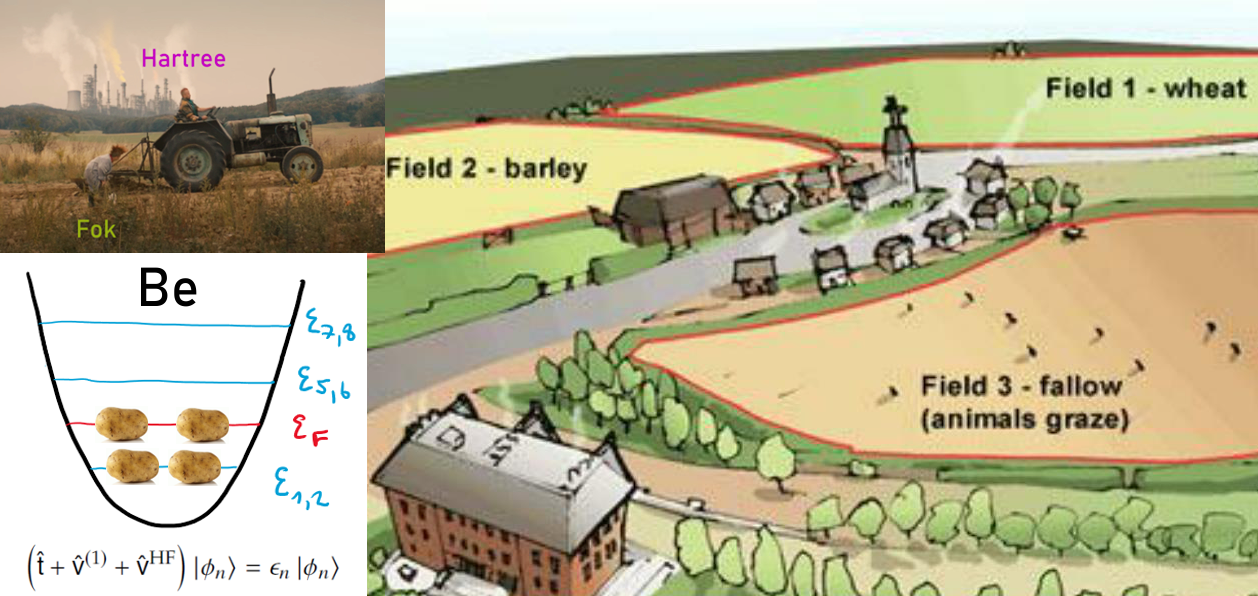
\includegraphics[width=\linewidth]{HF.png}
\end{figure}
